\section{Statistik}
\paragraph{Unterteilung der Statistik}
\begin{itemize}
	\item Beschreibende (deskriptive) Statistik: Aussagen werden auf den betrachteten Daten getroffen
	\item Beurteilende (schließende, induktive) Statistik: Aus vorliegenden Daten werden Rückschlüsse auf allgemeine Gültigkeit getroffen.  
\end{itemize}

\subsection{Deskriptive Statistik}
\paragraph{Definition: Stichprobe}
Sei $\XG$ die Menge aller Beobachtungen in einem Zufallsexperiment.
Bezeichne mit $x_i\in\XG$ das $i$-te Ergebnis, dann heißt $x\coloneqq(x_1,\ldots,x_n)$ \textbf{Stichprobe} vom Umfang $n\in\N$.
$\XG$ heißt \textbf{Stichprobenraum}.

\paragraph{Absolute und relative Häufigkeit}
Für $a\in\XG$ und eine Stichprobe $x$ ist die \textbf{absolute} bzw. \textbf{relative Häufigkeit} von $a$ in $x$ definiert durch
\begin{tightcenter}
	$H_x(a)\coloneqq\sum\limits_{i=1}^{n}\mathds{1}_{\{x_i=a\}}\qquad$ bzw. $\qquad h_x(a)\coloneqq\cfrac{H_x(a)}{n}$
\end{tightcenter}

\paragraph{Definition: Merkmal}
Die bei einem stochastischen Vorgang beobachtbaren Größen heißen \textbf{Merkmale}.
Werte, die von Merkmalen angenommen werden können, heißen \textbf{Merkmalsausprägungen}.

\paragraph{Definition: Empirische Verteilungsfunktion}
Die Funktion
\begin{tightcenter}
	$F_n:\R\rightarrow[0,1], \qquad t\mapsto F_n(t)\coloneqq\frac{1}{n}\sum\limits_{i=1}^{n}\mathds{1}_{\{x_i\leq t\}}$
\end{tightcenter}
heißt \textbf{empirische Verteilungsfunktion} von $x=(x_1,\ldots,x_n)$.
Für ein diskretes Merkmal gilt $F_n(t)=\sum_{a\leq t}h_x(a)$.

\newpage
\paragraph{Definition: Histogramm}
Das \textbf{Histogramm} ist definiert durch
\begin{tightcenter}
	$\hat{f}_n^{hist}\coloneqq\sum\limits_{k=1}^{K}d_k\mathds{1}_{(a_k,a_{k+1}]}(y)$,\qquad wobei
	\begin{itemize}
		\item $d_k\coloneqq\cfrac{n_k}{a_{k+1}-a_k}$ (Gewichtung nach Größe der Klasse)
		\item $n_k\coloneqq\frac{1}{n}\sum\limits_{i=1}^{n}\mathds{1}_{\{a_k<x_i\leq a_{k+1}\}}$ (Relative Häufigkeit der Klasse)
	\end{itemize}
\end{tightcenter}

\paragraph{Kenngrößen}
\begin{itemize}
	\item $\bar{x}\coloneqq\frac{1}{n}\sum\limits_{i=1}^{n}x_i$ \qquad(\textbf{Stichproben-Mittel})
	\item $s_x^2\coloneqq\frac{1}{n-1}\sum\limits_{i=1}^{n}(x_i-\bar{x})^2=\frac{1}{n-1}(\sum\limits_{i=1}^{n}x_i^2-n\cdot\bar{x}^2)$ \qquad(\textbf{Stichproben-Varianz})
	\item $s_x\coloneqq\sqrt{s_x^2}$ \qquad(\textbf{Stichprobenstandardabweichung})
	\item $v_x\coloneqq\cfrac{s_x}{\bar{x}}$ \qquad(\textbf{Stichprobenvariationskoeffizient})
	\item Sei $x_{()}\coloneqq(x_{(1)},\ldots,x_{(n)})$ eine aufsteigend sortierte Stichprobe.
	\[   
	\tilde{x}\coloneqq
	\begin{cases}
		x_{(\frac{n+1}{2})} & \qquad\text{falls n ungerade}\\
		\frac{1}{2}\cdot(x_{(\frac{n}{2})}+x_{(\frac{n}{2}+1)}) & \qquad\text{falls n gerade}
	\end{cases}
	\]
	heißt \textbf{Stichprobenmedian}.
	\item Für $p\in(0,1)$ und $k\coloneqq\lfloor n\cdot p\rfloor$ heißt
	\[   
	\tilde{x}_p\coloneqq
	\begin{cases}
		x_{(k+1)} & \qquad\text{falls }n\cdot p\notin\N\\
		\frac{1}{2}\cdot(x_{(k)}+x_{(k+1)}) & \qquad\text{sonst}
	\end{cases}
	\]
	das \textbf{Stichproben-$\boldsymbol{p}$-Quantil}.
	\item \textbf{Quartilsabstand}: $\tilde{x}_{0,75}-\tilde{x}_{0,25}$, \textbf{Stichprobenspannweite}: $x_{(n)}-x_{(1)}$,\\
	\textbf{Mittlere absolute Abweichung}: $\frac{1}{n}\sum\limits_{i=1}^{n}|x_i-\bar{x}|$
	\item Für $\alpha\in[0,0.5)$ und $k\coloneqq\lfloor n\cdot \alpha\rfloor$ ist $\bar{x}_\alpha\coloneqq\frac{1}{n-2\cdot k}\cdot(x_{(k+1)}+\ldots+x_{(n-k)})$ das \textbf{$\boldsymbol{\alpha}$-getrimmte Stichprobenmittel}.
\end{itemize}

\paragraph{Beschreibung zweidimensionaler Daten}
Ein \textbf{(parametrisches) Regressionsmodell} versucht die Beobachtungen mit einer Regressionsfunktion $f_\beta$ für ein geeignetes $\beta\in\R^p$ möglichst gut zu beschreiben, d.h. $y_i\approx f_\beta(x_i)$ für alle $i=1,\ldots,n$.

\paragraph{Einfache lineare Regression}
Die \textbf{Regressionsgerade} $y=a^*+b^*x$ ist bestimmt durch $a^*,b^*$ als Lösung von\\
$\min\limits_{a,b\in\R}\sum\limits_{i=1}^{n}(y_i-a-bx_i)^2$ (\textbf{Kleinste-Quadrate-Methode}).
Lösung ist gegeben durch
\begin{tightcenter}
	$b^*=\cfrac{\sum\limits_{j=1}^{n}(x_j-\bar{x})(y_i-\bar{y})}{\sum\limits_{j=1}^{n}(x_j-\bar{x})^2}$ \qquad und\qquad
	$a^*=\bar{y}-b^*\bar{x}$
\end{tightcenter}
Der \textbf{(empirische) (Pearson-) Korrelationskoeffizient} von $(x_1,y_1),\ldots,(x_n,y_n)$ ist gegeben durch
\begin{tightcenter}
	$r_{xy}=\cfrac{\frac{1}{n-1}\sum\limits_{j=1}^{n}(x_j-\bar{x})(y_j-\bar{y})}{s_xs_y}$
	$=\cfrac{\frac{1}{n-1}(\sum\limits_{j=1}^{n}x_j\cdot y_j-n\cdot\bar{x}\bar{y})}{s_xs_y}$
\end{tightcenter}
wobei $s_k$ die Stichprobenstandardabweichung von $k$ ist.
Damit gilt $b^*=r_{xy}\frac{s_y}{s_x}$.

\paragraph{Eigenschaften von $\boldsymbol{r_{xy}}$}
\begin{itemize}
	\item Es gilt $-1\leq r_{xy}\leq 1$
	\item Je nachdem ob $r_{xy}$ positiv oder negativ ist, liegt ein ansteigender oder fallender linearer Trend vor
	\item Bei linearen Datentransformationen der Form $\tilde{x}=a\cdot x_j+b$, $\tilde{y}=c\cdot y_j+d$ ändert sich $r_{xy}$ nicht, d.h. $r_{\tilde{x}\tilde{y}}=r_{xy}$
\end{itemize}

\subsection{Induktive Statistik}
\paragraph{Definition: Statistisches Experiment}
Ein messbarer Raum $(\XG,\FG)$ versehen mit einer Familie $(\PP_\vt)_{\vt\in\Theta}$ von Wahrscheinlichkeitsmaßen mit einer beliebigen \textbf{Parametermenge} $\Theta\neq\emptyset$ heißt \textbf{statistisches Experiment} oder \textbf{statistisches Modell}. 
Zufallsvariablen auf $(\XG,\FG,(\PP_\vt)_{\vt\in\Theta})$ heißen \textbf{Beobachtung} oder \textbf{Statistik}.

\paragraph{Definition: Unabhängige Stichprobe}
Die Stichprobe $x=(x_1,x_2,\ldots,x_n)$ heißt als Realisierung eines Zufallsvektors\\ 
$X=(X_1,X_2,\ldots,X_n)\in\XG$ \textbf{unabhängige Stichprobe}, wenn alle $X_i$ identisch und unabhängig verteilt sind.
Hat diese Stichprobe eine Randverteilungsdichte $X_1\sim f_\vt$, so ist der Stichprobenvektor verteilt mit $f_\vt^n(x_1,\ldots,x_n)=\prod\limits_{i=1}^{n}f_i(x_i)$\\

\underline{Bemerkung}: Kenngrößen wie $\E_\vt$ oder $Var_\vt$ von $\PP_\vt$ hängen von $\vt$ ab.

Mit einer gegebenen Stichprobe sollen Aussagen über die zugrunde liegende Verteilung $\PP_\vt$ gemacht werden.
Parameterschätzung, Hypothesentests und Konfidenzbereiche sind grundlegende Kategorien zur Untersuchung.

\paragraph{Definition: Schätzer}
Sei $(\XG,\FG,(\PP_\vt)_{\vt\in\Theta})$ ein statistisches Modell, $\rho:\Theta\rightarrow\R^d$ ein $d$-dimensionaler Parameter.
Ein \textbf{Schätzer} ist eine Abbildung $\hat{\rho}:\XG\rightarrow\R^d$.
Gilt $\E_\vt[\hat{\rho}]=\rho(\vt)$, so heißt $\hat{\rho}$ \textbf{unverzerrt} oder \textbf{erwartungstreu}.

\paragraph{Definition: Verlust und Risiko}
Eine Funktion $l:\Theta\times\R^d\rightarrow\R_+$ heißt \textbf{Verlustfunktion}, falls $l(\vt,\cdot)$ für alle $\vt\in\Theta$ messbar ist.
Der erwartete Verlust $R(\vt,\hat{\rho})\coloneqq\E_\vt[l(\vt,\hat{\rho})]$ eines Schätzers $\hat{\rho}$ heißt \textbf{Risiko}.
Besonders wichtig ist der \textbf{quadratische Verlust}: $l(\vt,r)=|r-\rho(\vt)|^2$.

\paragraph{Bias-Varianz-Zerlegung}
Sei $(\XG,\FG,(\PP_\vt)_{\vt\in\Theta})$ ein statistisches Modell und $\hat{\rho}:\XG\rightarrow\R^d$ ein Schätzer des Parameters $\rho(\vt)$ mit $\E_\vt[|\hat{\rho}|^2]<\infty$.
Dann gilt für den quadratischen Verlust:
\begin{tightcenter}
	$\E_\vt[|\hat{\rho}-\rho(\vt)|^2]=Var_\vt(\hat{\rho})+|\E_\vt[\hat{\rho}]-\rho(\vt)|^2$
\end{tightcenter}
Der hintere Summand ist der \textbf{Bias}.

\paragraph{Definitionen für asymptotische Eigenschaften von Schätzern}
Seien $X_1,\ldots,X_n\sim\PP_\vt$ eine i.i.d Stichprobe.
Dann heißt eine Folge von Schätzern $\hat{\rho}=\hat{\rho}(X_1,\ldots,X_n)$ für den abgeleiteten Parameter $\rho(\vt)\in\R$
\begin{itemize}
	\item \textbf{asymptotisch konsistent}, falls $\hat{\rho}_n\xrightarrow{\PP_\vt}\rho(\vt)$ für $n\rightarrow\infty$
	\item \textbf{asymptotisch erwartungstreu}, falls $\E_\vt[\hat{\rho}_n]\rightarrow\rho(\vt)$ für $n\rightarrow\infty$
	\item \textbf{asymptotisch normalverteilt}, falls $\E_\vt[|\hat{\rho}_n|^2]<\infty$ und
	$\PP_\vt(\cfrac{\hat{\rho}_n-\E_\vt[\hat{\rho}_n]}{\sqrt{Var_\vt(\hat{\rho}_n)}}\leq t)\rightarrow\Phi(t)$ für $n\rightarrow\infty$ und alle $t\in\R$
\end{itemize}

Wir wollen im Folgenden Schätzer konstruieren.

\paragraph{Empirische Maßzahlen}
Schätze Maßzahlen durch deren empirisches Analogon einer unabh. Stichprobe:
\begin{center}
	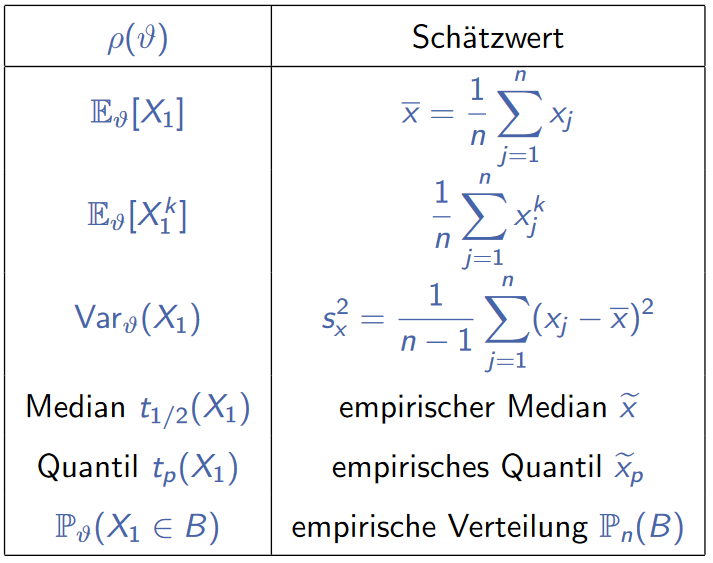
\includegraphics[width=0.5\textwidth]{images/image4.png}
\end{center}
Für diese Schätzmethode braucht man kein parametrisches Modell.

\paragraph{Erwartungstreue von empirischen Maßzahlen}
Folgende Schätzer sind für eine unabhängige Stichprobe erwartungstreu:
\begin{itemize}
	\item $\overline{X}_n\coloneqq\frac{1}{n}\sum\limits_{j=1}^{n}X_j$ erwartungstreu für $\E_\vt[X_1]$
	\item $\PP_n(B)\coloneqq\frac{1}{n}\sum\limits_{j=1}^{n}\{X_j\in B\}$ erwartungstreu für $\PP(X_1\in B)$ für jede Borelmenge $B\in\BG_\R$
	\item $s_n^2(X_1,\ldots,X_n)\coloneqq\frac{1}{n-1}\sum\limits_{j=1}^{n}(X_j-\overline{X}_n)^2$ erwartungstreu für $Var_\vt(X_1)$
\end{itemize}
Mit dem zentralen Grenzwertsatz folgt die Konsistenz der obigen Werte.

\paragraph{Momentenmethode}
\begin{itemize}
	\item Seien $X_1,\ldots,X_n$ i.i.d. verteilte Zufallsvariablen
	\item Gegeben Verteilung versuche die Parameter zu schätzen
	\item Bestimme die ersten $k$ Momente $m_k(\vt)\coloneqq\E_\vt[X_1^k]$
	\item Schätze $m_k(\vt)$ durch das $k$-te Stichprobenmoment $\hat{m}_k(x)=\frac{1}{n}\sum\limits_{j=1}^{n}x_j^k$
	\item \textbf{Momentenschätzer} ergibt sich durch Auflösen der Gleichungen $m_k(\vt)=\hat{m}_k(x)$
\end{itemize}

\paragraph{Definition: Maximum-Likelihood-Schätzer}
\begin{itemize}
	\item Für eine feste Stichprobe $x=(x_1,\ldots,x_n)$ heißt $\Theta\ni\vt\mapsto L_x(\vt)\coloneqq\prod\limits_{j=1}^{n}f_\vt(x_j)$ die \textbf{Likelihood-Funktion} zu $x$.
	\item Der Wert $\hat{\vt}\in\Theta$ an dem $L_x(\cdot)$ einen Maximalwert annimmt heißt \textbf{Maximum-Likelihood-Schätzwert} von $\vt$ zu $x$. Der Schätzer $\hat{\vt}:\XG\rightarrow\Theta$ heißt \textbf{Maximum-Likelihood-Schätzer}.
\end{itemize}
Berechnung:
\begin{itemize}
	\item Maximieren der Likelihood-Funktion ist äquivalent zur Maximierung der Loglikelihood-Funktion: $l_x(\vt)\coloneqq\sum\limits_{i=1}^n\log f_\vt(x_i)$
	\item Finde Maximum durch die Ableitung.
\end{itemize}
